\chapter{Cơ sở lý thuyết}
\section{Công nghệ RFID và quá trình phát triển}
\subsection{Giới thiệu công nghệ RFID}
Công nghệ RFID (Radio Frequency Identification) cho phép một thiết bị đọc thông tin chứa trong chip không cần tiếp xúc trực tiếp ở khoảng cách xa,
không thực hiện bất kì giao tiếp vật lý giữa hai vật không nhìn thấy nhau.
Công nghệ này cho phép truyền, nhận dữ liệu từ một điểm này đến một điểm khác không cần tiếp xúc (contactless communication).

Kỹ thuật RFID sử dụng truyền thông không dây trong dải tần sóng vô tuyến từ để truyền dữ liệu từ các thẻ (tag) đến bộ đọc (reader).
Tag có thể được đính kèm hoặc gắn vào đối tượng được nhận dạng.
Reader đọc dữ liệu của tag và gửi thông tin đến cơ sở dữ liệu có lưu trữ dữ liệu của tag.
Các chip không tiếp xúc, không tích điện sẵn, chúng hoạt động nhờ năng lượng thu nhận từ tín hiệu gửi bởi reader.

Đề tài này sử dụng công nghệ RFID đơn giản nhất hiện nay là hệ thống RFID bị động làm việc như sau:
reader truyền một tín hiệu tần số vô tuyến từ anten của nó đến một chip.
Reader nhận thông tin trở lại từ chip và gửi nó đến mạch điều khiển đầu đọc và xử lý thông tin lấy được từ chip.
\subsection{Lược sử và quá trình phát triển}
- Năm 1897: Guglielmo Marconi phát hiện ra sóng radio, tạo nền tảng đểphát triển RFID.

- Năm 1937: Phòng thí nghiệm nghiên cứu Naval US phát triển hệ thống Friend-or-Foe (IFF) cho phép nhận diện các đối tượng thuộc về quân ta hay quân địch.

- Trong suốt thập niên 50: Công nghệ IFF chủ yếu được dùng trong quân đội, các phòng lab nghiên cứu.
Thiết bị trong giai đoạn này có kích thước lớn và giá thành rất cao, không thể áp dụng được trong môi trường doanh nghiệp.
\begin{figure}[ht]
\centering
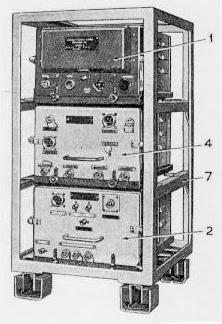
\includegraphics[scale=0.9]{images/interrogator_242.jpg}
\caption{Interrogator 242}
\end{figure}

- Cuối thập niên 60, đầu thập niên 70: Nhiều công ty như Sensormatic and Checkpoint Systems giới thiệu những sản phẩm mới ít phức tạp hơn và có thể ững dụng rộng rãi hơn do công nghệ mới này được tích hợp sẵn IC, chip nhớ lập trình được.
Các công ty bắt đầu phát triển thiết bị giám sát điện tử để bảo vệ và kiểm kê sản phẩm như quần áo trong cửa hàng, sách trong thư viện, v.v..
Hệ thống RFID thương mại ban đầu này chỉ là hệ thống tag 1-bit giá rẻ để xây dựng, thực hiện và bảo hành.
Tag không đòi hỏi nguồn pin (thụ động) dễ dàng đặt vào sản phẩm và thiết kế để cảnh bảo khi tag đến gần reader,
thường đặt tại lối ra vào để phát hiện sự có mặt của tag.

- Suốt thập niên 70: Có nhiều nghiên cứu và phát triển các dự án để phát minh nhiều IC mới sử dụng công nghệ RFID.
Có nhiều ứng dụng mới trong công nghiệp tự động như xác định thú vật, theo dõi lưu thông.
Tag có đặc điểm mới: bộ nhớ ghi được, tốc độ đọc nhanh hơn và khoảng cách đọc xa hơn.

- Đầu thập niên 80: Được áp dụng rộng rãi trong nhiều ứng dụng: đặt tại nhiều đường ray ở Mỹ,
đánh dấu thú vật ở các nông trại mô hình lớn ở châu Âu.
Hệ thống RFID còn dùng trong nghiên cứu động vật hoang dã hoặc đánh dấu các loài thú quý hiếm hay có nguy cơ tuyệt chủng.

- Đầu thập niên 90: Xuất hiện nhiều hệ thống thu phí điện tử, tiêu chuẩn hóa các đặt tính kỹ thuật như tần số hoạt động
và giao tiếp phần cứng.

\newpage
- Cuối thế kỷ 20: Phát triển nhanh trên phạm vi toàn cầu.
EPCGlobal được thành lập và hỗ trợ hệ thống mã sản phẩm điện tử (Electronic Product Code - EPC)
và hệ thống này đã trở thành tiêu chuẩn cho xác nhận sản phẩm tự động.

\subsection{Thành phần một hệ thống RFID}
\begin{figure}[ht]
\centering
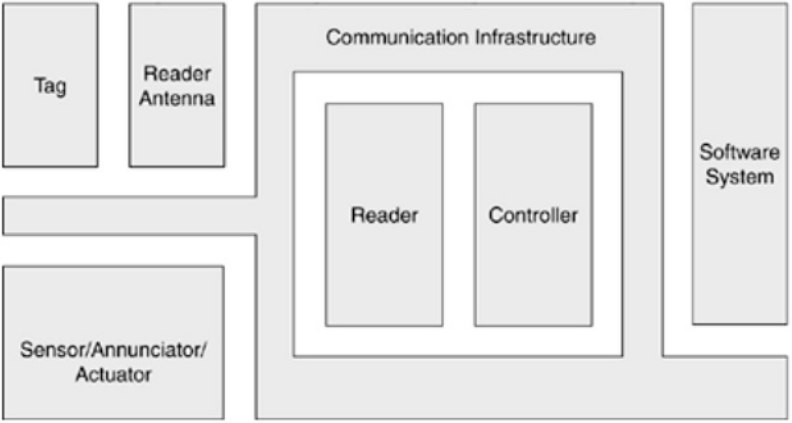
\includegraphics[scale=0.6]{images/rfid_block_diagram.png}
\caption{Sơ đồ khối một hệ thống RFID}
%\label{fig:rfid_block_diagram}
\end{figure}
%Hình \ref{fig:rfid_block_diagram} là mô hình một hệ thống RFID cơ bản.

Một hệ thống RFID là bao gồm các thành phần cơ bản sau:
\begin{itemize}
    \item \textbf{Reader}: Là thành phần bắt buộc, thực hiện việc đọc, ghi dữ liệu lên tag, giao tiếp với mạch điều khiển.
    \item \textbf{Anten}: Làm nhiệm vụ bức xạ, thu sóng điện tử và gia công tín hiệu.
    \item \textbf{Mạch điều khiển}: Là thành phần bắt buộc, tuy nhiên hầu hết các reader hiện đại đều có IC tích hợp.
        Cho phép các thành phần bên ngoài như con người, chương trình máy tính giao tiếp điều khiển các chức năng của reader, annunciator, cơ cấu chấp hành kết hợp với reader.
    \item \textbf{Cảm biến} (sensor), \textbf{cơ cấu chấp hành} (actuator) và \textbf{bảng tín hiệu điện báo} (annunciator): hỗ trợ xuất và nhập hệ thống.
    \item \textbf{Máy chủ/Hệ thống phần mềm}: Về mặt lý thuyết, một hệ thống RFID có thể hoạt động mà không cần đến thành phần này.
        Tuy nhiên trong thực tế, một hệ thống RFID gần như không có ý nghĩa nếu không có thành phần này.
    \item \textbf{Cơ sở hạ tầng truyền thông}: Là thành phần bắt buộc, nó là tập hợp gồm cả 2 mạng có dây và không dây và các bộ phận kết nối tuần tự để kết nối các thành phần đã liệt kê ở trên lại với nhau để hoạt động hiệu quả.
\end{itemize}

\subsection{Phương thức làm việc của RFID}
Một hệ thống RFID có ba thành phần cơ bản: tag, đầu đọc, và một máy chủ.
Mỗi tag được lập trình với một nhận dạng duy nhất cho phép theo dõi không dây đối tượng hoặc con người đang gắn tag đó.
Bởi vì các chip được sử dụng trong tag RFID có thể giữ một số lượng lớn dữ liệu,\
chúng có thể chứa thông tin như chuỗi số, thời dấu, hướng dẫn cấu hình, dữ liệu kỹ thuật, sổ sách y học, và lịch trình.
Cũng như phát sóng tivi hay radio, hệ thống RFID cũng sử dụng bốn băng thông tần số chính:
tần số thấp (LF), tần số cao (HF), siêu cao tần (UHF) hoặc sóng cực ngắn (viba).
Các hệ thống trong siêu thị ngày nay hoạt động ở băng thông UHF,
trong khi các hệ thống RFID cũ sử dụng băng thông LF và HF.
Băng thông viba đang được để dành cho các ứng dụng trong tương lai.

Các tag có thể được cấp nguồn bởi một bộ pin thu nhỏ trong tag (các tag tích cực)
hoặc bởi reader mà nó ``wake up'' (đánh thức) tag để yêu cầu trả lời khi tag đang trong phạm vi (tag thụ động).
Hình \ref{fig:tag_reader_workflow} là mô hình hoạt động giữa tag và reader RFID.
\begin{figure}[ht]
\centering
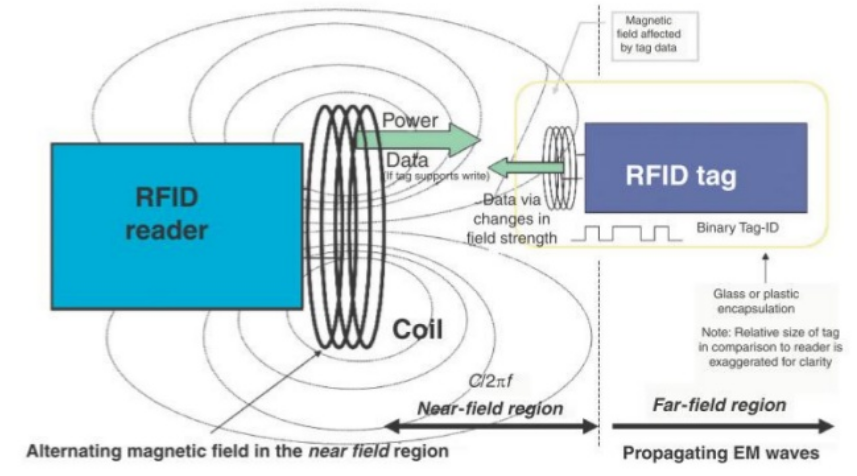
\includegraphics[scale=0.5]{images/tag_reader_workflow.png}
\caption{Hoạt động giữa tag và reader RFID}
\label{fig:tag_reader_workflow}
\end{figure}

Tag tích cực đọc xa 100 feet tính từ reader và có thể là tag RW (với bộ nhớ được viết lên và xóa như một ổ cứng máy tính) hoặc là tag RO.
Tag thụ động có thể được đọc xa reader 20 feet và có bộ nhớ RO.
Kích thước tag, giá cả, dải đọc, độ chính xác đọc/ghi, tốc độ dữ liệu và chức năng hệ thống thay đổi theo đặc điểm nêu ra trong thiết kế và dải tần hệ thống FRID sử dụng.

Reader gồm một anten liên lạc với tag và một đơn vị đo điện tử học đã được nối mạng với máy chủ.
Đơn vị đo tiếp sóng giữa máy chủ và tất cả các tag trong phạm vi đọc của anten, cho phép một đầu đọc liên lạc đồng thời với hàng trăm tag.
Nó cũng thực thi các chức năng bảo mật như mã hóa/giải mã và xác thực người dùng.
Reader có thể phát hiện tag ngay cả khi không nhìn thấy chúng.
Hầu hết các mạng RFID gồm nhiều tag và nhiều đầu đọc được nối mạng với nhau bởi một máy tính trung tâm, hầu như thường là một trạm làm việc gọn để bàn.
Máy chủ xử lý dữ liệu mà các reader thu thập từ các tag và dịch nó giữa mạng RFID và các hệ thống công nghệ thông tin lớn hơn,
mà nơi đó quản lý dây chuyền hoặc cơ sở dữ liệu quản lý có thể thực thi.
Middleware là phần mềm nối hệ thống RFID với một hệ thống IT quản lý luồng dữ liệu.

\subsection{Một số ứng dụng thực tế của RFID}
Công nghệ RFID hiện nay được áp dụng rộng rãi trên rất nhiều lĩnh vực khác nhau, sau đấy là một số ứng dụng cụ thể.

- Bảo mật, an ninh:
\begin{itemize}
    \item Điều khiển truy nhập (access control): khóa và các thiết bị cố định.
    \item Quy trình quản lý.
    \item Chống trộm trong kinh doanh và mua bán hàng hóa nói chung.
\end{itemize}
- Giám sát:
\begin{itemize}
    \item Dây chuyền cung cấp: điều khiển kiểm soát trong các nhà kho.
    \item Người hoặc động vật: trẻ em, bệnh nhân, động vật quý hiếm.
    \item Tài sản, hành lý trên máy bay, hoặc trong vận chuyển hàng hóa.
\end{itemize}
- Các hệ thống tự động:
\begin{itemize}
    \item Lưu thông: hệ thống thu phí tự động.
    \item Hệ thống điểm danh tự động.
    \item Hệ thống xử lý thẻ xe tự động.
\end{itemize}

\section{Giới thiệu phần cứng}
\subsection{Evaluation kit EK-TM4C123G}
\subsubsection{Giới thiệu kit}
\begin{figure}[ht]
\centering
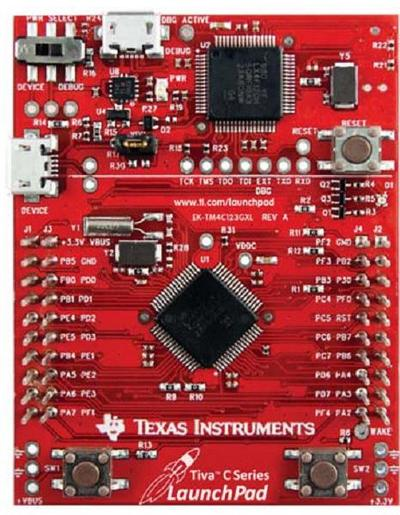
\includegraphics[scale=0.5]{images/kit_tivac.jpg}
\caption{Evaluation kit EK-TM4C123G}
\end{figure}

Evaluation kit EK-TM4C123G (từ đây tôi xin được gọi tắt là kit TIVA C) là một vi điều khiển có kích thước chỉ bằng một thẻ ATM thông dụng.
Kit TIVA C được phát triển bởi tập đoàn Texas Instrument (TI) để thay thế cho sản phẩm Stellaris Launchpad đã dừng sản xuất trước đó.
Dòng TIVA C 32-bit được sử dụng trong đề tài này có một thiết kế hiện đại cùng tập lệnh phong phú và hệ sinh thái về code nhúng giàu có
đã đẩy nhanh việc giảng dạy về lập trình nhúng nói chung trong môi trường trường học cũng như cũng đủ mạnh mẽ để có thể phát triển thêm lên để sử dụng trong môi trường công nghiệp hiện đại.

Kit TIVA C xây dựng xoay quanh bộ xử lý có kiến trúc ARM-Cortex M4F có tốc độ lên đến \si{80\MHz}, có kèm theo bộ tính toán dấu chấm động FPU, nhiều bộ nhớ tích hợp, nhiều chân lập trình GPIO, cũng như nhiều tính năng khác.
Kit TIVA C là một giải pháp hoàn hảo với chi phí thấp để thực hiện những đề tài về lập trình nhúng trong môi trường trường học.

Một số ứng dụng tiêu biểu sử dụng kit TIVA C có thể nêu ra như: xử lý âm thanh giọng nói, điều khiển thiết bị cầm tay, điều khiển nhà thông minh, điều khiển thiết bị y tế, v.v..

Trong đề tài này tôi chọn dòng EK-TM4C123G (cụ thể ở đây là EK-TM4C123GH6PM) là kit phát triển thông dụng nhất của dòng TIVA C được tập đoàn TI sản xuất.

\subsubsection{Thông tin cấu hình kit TIVA C}
\begin{figure}[ht]
\centering
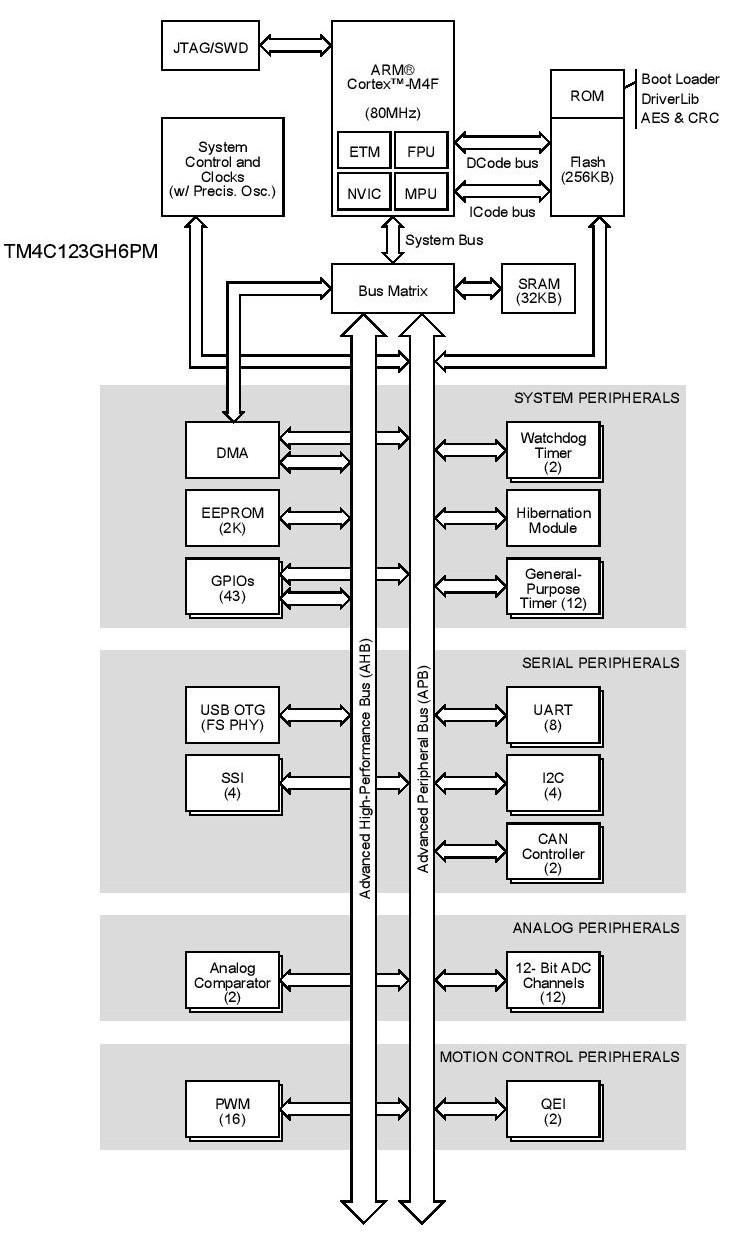
\includegraphics[scale=0.45]{images/tiva_c_diagram.jpg}
\caption{Sơ đồ khối kit TIVA C}
\end{figure}

\textbf{Cấu hình kit TIVA C}
\begin{itemize}
\item Vi xử lý: kiến trúc ARM Cortex-M4F tốc độ lên đến \si{80\MHz} kèm FPU, 100 DMIPS.
\item SRAM: 32KB
\item Bộ nhớ Flash: 256KB
\item EEPROM: 2KB
\end{itemize}

\textbf{Các tính năng nổi bật của kit TIVA C}
\begin{itemize}
\item 6 khối GPIO (A, B, C, D, E, F)
\item 2 modules 12-bit ADC
\item 8 UARTs
\item 4 SSI modules
\item 4 I\textsuperscript{2}C modules
\end{itemize}

\textbf{Ưu điểm}: Giá thành rẻ, nhỏ gọn, mạnh mẽ. Có bộ thư viện phong phú dễ dàng thực hiện lập trình nhúng trên nhiều lĩnh vực.
Khả năng hoạt động với chế độ tiết kiệm điện để hoạt động liên tục, phù hợp cho việc áp dụng cho môi trường thực tiễn.

\textbf{Nhược điểm}: Giá thành vẫn còn đắt hơn so với một số thiết bị dòng STM32, không có tích hợp GPU nên rất khó để lập trình nhúng liên quan đến xử lý ảnh nói chung.

\subsection{LCD 1602 Display Module}
\subsubsection{Giới thiệu LCD 1602}
\begin{figure}[ht]
\centering
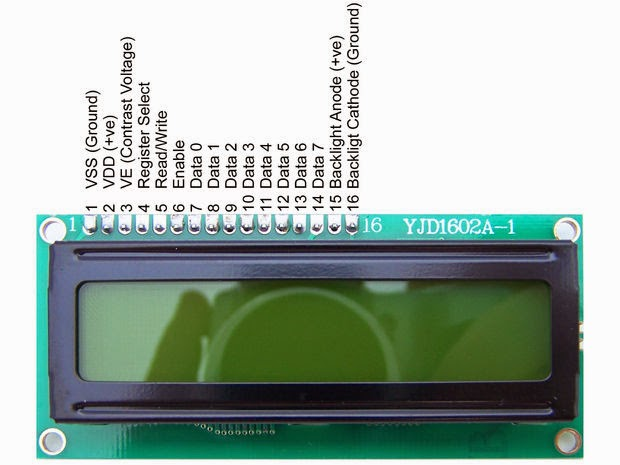
\includegraphics[scale=0.45]{images/lcd1602.jpg}
\caption{LCD 1602}
\label{fig:lcd1602}
\end{figure}

Liquid Crystal Displaly (LCD) được sử dụng rộng rãi trong nhiều ứng dụng điện tử.
LCD 1602 tức là có 2 dòng kí tự với đối đa 16 kí tự trên mỗi dòng.
Có rất nhiều loại LCD với hình dáng, kích thước, cách sử dụng khác nhau, ở hình \ref{fig:lcd1602} là loại LCD 1602 thông dụng nhất diện nay.
Khi sản xuất LCD, nhà sản xuất đã tích hợp chip điều khiển (HD44780) trên trong lớp vỏ và đã ra các chân giao tiếp cần thiết trên module này.
Các chân này được đánh số thứ tự và đặt tên như hình \ref{fig:lcd1602}.

\newpage
\textbf{Thông số LCD 1602}:
\begin{itemize}
\item Điện áp MAX: \si{7\volt}
\item Điện áp MIN: \si{\num{-0.3}\volt}
\item Điện áp hoạt động: \SIrange[range-phrase=--, range-units=single]{2.7}{5.5}{\volt}
\item Dòng điện cấp nguồn: \SIrange[range-phrase=--, range-units=single]{350}{600}{\micro\ampere}
\item Nhiệt độ hoạt động: \SIrange[range-phrase=--, range-units=single]{-30}{75}{\celsius}
\end{itemize}

\begin{longtable}{l l p{0.7\textwidth}} \toprule
Chân & Ký hiệu & Mô tả \\
\midrule
\endhead
1 & VSS & Chân nối đất cho LCD, khi thiết kế mạch nối chân này với GND của mạch điều khiển \\ \midrule
2 & VDD & Chân cấp nguồn cho LCD, khi thiết kế mạch nối chân này với chân cấp nguồn \si{5\volt} của mạch điều khiển \\ \midrule
3 & V0 & Điều chỉnh độ tương phản của LCD \\ \midrule
4 & RS & Chân chọn thanh ghi (Register Select). Nối chân RS với logic ``0'' (GND) hoặc logic ``1'' (VCC) để chọn thanh ghi.\newline
- Logic ``0'': Bus DB0--DB7 sẽ nối với thanh ghi lệnh IR của LCD (ở chế độ ``ghi'' - write) hoặc nối với bộ đếm địa chỉ của LCD (ở chế độ ``đọc'' - read)\newline
- Logic ``1'': Bus DB0--DB7 sẽ nối với thanh ghi dữ liệu bên trong LCD. \\ \midrule
5 & R/W & Chân chọn chế độ đọc/ghi (read/write). Nối chân R/W với logic ``0'' để LCD hoạt động ở chế độ ghi, hoặc nối với logic ``1'' để LCD hoạt động ở chế độ đọc. \\ \midrule
6 & E & Chân cho phép hoạt động (Enable). Sau khi các tín hiệu được đặt lên bus DB0--DB7, các lệnh chỉ được chấp nhận khi có 1 xung cho phép của chân E.\newline
- Ở chế độ ghi: Dữ liệu ở bus sẽ được LCD chuyển vào (chấp nhận) thanh ghi bên trong nó khi phát hiện một cạnh xuống (high-to-low transistion) của tín hiệu E.\newline
- Ở chế độ đọc: Dữ liệu sẽ được LCD xuất ra DB0--DB7 khi phát hiện cạnh lên (low-to-high transistion) ở chân E và được LCD giữ ở bus đến khi nào chân E xuống mức thấp. \\ \midrule
7--14 & DB0--DB7 & 8 đường của bus dữ liệu dùng để trao đổi thông tin với mạch điều khiển. Có 2 chế độ sử dụng 8 đường bus này:\newline
- Chế độ 8-bit: Dữ liệu được truyền trên cả 8 đường, với MSB là bit DB7.\newline
- chế độ 4-bit: Dữ liệu được truyền hai lần trên 4 đường DB4--DB7, với bit MSB là DB7. \\ \midrule
15 & --- & Nguồn cấp cho đèn nền của LCD. \\ \midrule
16 & --- & Chân GND cho đèn nền của LCD. \\
\bottomrule
\caption{Chức năng các chân của LCD 1602}
\end{longtable}
\textbf{Ghi chú}:\newline
Ở chế độ ``đọc'', nghĩa là mạch điều khiển đọc thông tin từ LCD thông qua các chân DBx.
Còn khi ở chế độ ``ghi'', nghĩa là mạch điều khiển xuất thông tin điều khiển cho LCD thông qua các chân DBx.

\subsubsection{Các chân điều khiển việc đọc ghi vào LCD 1602}
\begin{itemize}
    \item \textbf{RS (chân số 3)}:
\end{itemize}
Chân lựa chọn thanh ghi (Select Register), chân này cho phép lựa chọn 1 trong 2 thanh ghi IR hoặc DR để làm việc.
Vì cả 2 thanh ghi này đều được kết nối với các chân Data của LCD nên cần 1 bit để lựa chọn giữa chúng.
Nếu \(RS = 0\), thanh ghi IR được chọn và nếu \(RS = 1\) thanh ghi DR được chọn.

Chúng ta đều biết thanh ghi IR là thanh ghi chứa mã lệnh cho LCD,
vì thế nếu muốn gởi 1 mã lệnh đến LCD thì chân RS phải được reset về 0.
Ngược lại, khi muốn ghi mã ASCII của ký tự cần hiển thị lên LCD thì chúng ta sẽ set \(RS = 1\) để chọn thanh ghi DR.
\begin{itemize}
    \item \textbf{R/W (chân số 4)}:
\end{itemize}
Chân lựa chọn giữa việc đọc và ghi.
Nếu \(R/W = 0\) thì dữ liệu sẽ được ghi từ mạch điều khiển vào LCD.
Nếu \(R/W = 1\) thì dữ liệu sẽ được đọc từ LCD ra ngoài.
Tuy nhiên, chỉ có duy nhất 1 trường hợp mà dữ liệu có thể đọc từ LCD ra,
đó là đọc trạng thái LCD để biết LCD có đang bận hay không \emph{cBusyFlag - BF} .
Do LCD là một thiết bị hoạt động tương đối chậm (so với vi điều khiển),
vì thế một cờ BF được dùng để báo LCD đang bận, nếu \(BF = 1\) thì chúng ta phải chờ cho LCD xử lí xong nhiệm vụ hiện tại,
đến khi nào \(BF = 0\) một thao tác mới sẽ được gán cho LCD.
Vì thế, khi làm việc với Text LCD chúng ta nhất thiết phải có một chương trình con nào đó để chờ cho đến khi LCD rảnh.

Có 2 cách để viết chương trình \emph{waitLCD}.
Cách 1 là đọc bit BF về kiểm tra và chờ \(BF = 0\),
cách này đòi hỏi lệnh đọc từ LCD về bộ điều khiển ngoài, do đó chân R/W cần được nối với bộ điều khiển ngoài.
Cách 2 là viết một hàm delay một khoảng thời gian cố định nào đó. %(tốt nhất là trên \si{1\ms}).
Ưu điểm của cách 2 là sự đơn giản vì không cần đọc LCD, do đó chân R/W không cần sử dụng và luôn được nối với GND.
Tuy nhiên, nhược điểm của cách 2 là khoảng thời gian delay cố định nếu quá lớn sẽ làm chậm quá trình thao tác LCD,
nếu quá nhỏ sẽ gây ra lỗi hiển thị.
\begin{itemize}
    \item \textbf{E (chân số 5)}:
\end{itemize}
Chân cho phép LCD hoạt động (Enable), chân này cần được kết nối với bộ điều khiển để cho phép thao tác LCD.
Để đọc và ghi data từ LCD chúng ta cần tạo một xung cạnh xuống trên chân EN,
nói theo cách khác, muốn ghi dữ liệu vào LCD trước hết cần đảm bảo rằng chân \(EN = 0\),
tiếp đến xuất dữ liệu đến các chân DB0 đến DB7, sau đó set chân EN lên 1 và cuối cùng là xóa EN về 0 để tạo 1 xung cạnh xuống.

\subsection{Module đọc ghi thẻ MFRC522}
MFRC522 là một module chuyên dụng cho việc đọc/ghi thẻ có kết nối không dây.
Module hoạt động ở tần số \si{\num{13.56}\mega\hertz}.
Module hỗ trợ việc đọc/ghi vào các thẻ NFC (Near-Field Communications) hay còn gọi nôm na là
thẻ từ (loại thẻ thông dụng sử dụng để làm thẻ giảm giá, thẻ xe bus, tàu điện ngầm, v.v..).
MFRC522 hỗ trợ đọc/ghi thẻ kết nối không dây sử dụng công nghệ truyền tải MIFARE tốc độ cao lên đến \si{848}{kBd} cả hai hướng.

Ở hình \ref{fig:rc522} là hình dáng của module đọc ghi thẻ MFRC522 thông dụng nhất hiện nay.
Khi sản xuất module, nhà sản xuất đã tích hợp chip điều khiển (HVQFN32) và ra các chân giao tiếp cần thiết trên module này.
Các chân này được đánh dấu như trên hình \ref{fig:rc522}.
\begin{figure}[ht]
\centering
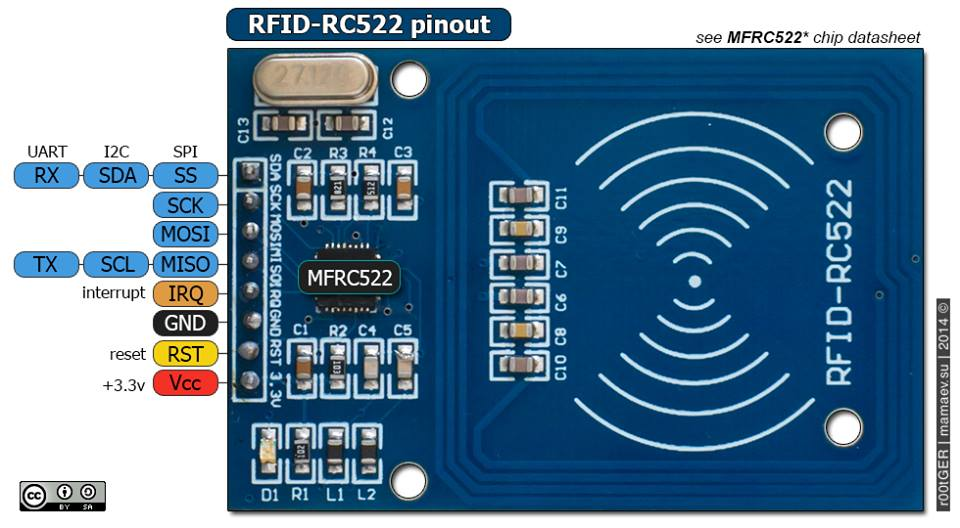
\includegraphics[scale=0.35]{images/rc522.jpg}
\caption{Module đọc ghi thẻ MFRC522}
\label{fig:rc522}
\end{figure}

\newpage
Module MFRC522 hỗ trợ giao tiếp thông qua các giao thức phổ biến như SPI, I\textsuperscript{2}C hay UART.
Module reset và kiểm tra lại giao thức giao tiếp tự động sau khi có nguồn cấp hoặc hard reset.
Module kiểm tra giao thức hoạt động của mạch điều khiển qua mức logic của các pin được kết nối sau giai đoạn reset
bằng cách kiểm tra cách kết nối của các pin dựa theo bảng \ref{tab:RC522_interface}.

\begin{longtable}{p{0.1\textwidth} p{0.2\textwidth} p{0.2\textwidth} p{0.2\textwidth}} \toprule
\multirow{2}{0.1\textwidth}{Pin} & \multicolumn{3}{l}{Giao thức} \\
\cline{2-4}
& UART (Input) & SPI (Output) & I\textsuperscript{2}C (I/O) \\
\midrule
\endhead
SDA & RX & NSS & SDA \\
I2C & 0 & 0 & 1 \\
EA & 0 & 1 & EA \\
D7 & TX & MISO & SCL \\
D6 & MX & MOSI & ADR\_0 \\
D5 & DTRQ & SCK & ADR\_1 \\
D4 & --- & --- & ADR\_2 \\
D5 & --- & --- & ADR\_3 \\
D6 & --- & --- & ADR\_4 \\
D7 & --- & --- & ADR\_5 \\
\bottomrule
\caption{Cách kết nối các chân module MFRC522}
\label{tab:RC522_interface}
\end{longtable}

Trong đề tài này, tôi chọn ứng dụng RFID bị động,
nên đã chọn giao thức giao tiếp SPI để giao tiếp với kit TIVA C
vì tốc độ truyền tải dữ liệu của giao thức SPI là rất nhanh (tốc độ truyền tải lên đến \si{10}{Mbps}).

\newpage
\section{Giới thiệu các giao thức giao tiếp}
\subsection{Giao thức SPI}
Giao thức SPI (Serial Peripheral Interface) là một trong những giao thức giao tiếp phổ biến nhất hiện nay,
nó được dùng để giao tiếp với vi điều khiển hoặc các ICs như cảm biến, ADC, DAC, SRAM, v.v..
Giao thức SPI hỗ trợ truyền tải tốc độ cao lên đến \si{10}{Mbps}.

Giao thức SPI là một loại giao thức kiểu Master -- Slave trong quan hệ đa điểm.
Trong loại giao diện này, một thiết bị được coi là master (thường là vi điều khiển) và tất cả các thiết bị khác (IC ngoại vi hoặc các vi điều khiển khác) được coi là slave.

Trong giao thức SPI, chỉ có thể có một thiết bị master nhưng có thể có nhiều thiết bị slave.
Bus SPI gồm 4 tín hiệu hoặc chân, chúng là:
\begin{itemize}
    \item Master-Out/Slave-In (\textbf{MOSI} hay SI): Cổng ra của master, cổng vào của slave, dành cho việc truyền dữ liệu của từ thiết bị master đến thiết bị slave.
    \item Master-In/Slave-Out (\textbf{MISO} hay SO): cổng vào của master, cổng ra của slave, dành cho việc truyền dữ liệu từ thiết bị slave đến thiết bị master.
    \item Serial Clock (\textbf{SCK} hay \textbf{SCLK}): xung nhịp cho giao tiếp SPI.
    \item Chip Select (\textbf{CS} hay Slave Select (\textbf{SS}): chọn chip.
\end{itemize}

Bởi vì bus SPI được thực hiện bằng cách sử dụng 4 tín hiệu hay 4 dây
nên đôi khi nó được gọi là chuẩn giao tiếp 4 dây (four-wire).
Hình \ref{fig:SPI_1M1S} mô tả một thiết bị master (vi xử lý) được kết nối với thiết bị slave (ngoại vi) sử dụng giao thức SPI.

\begin{figure}[ht]
\centering
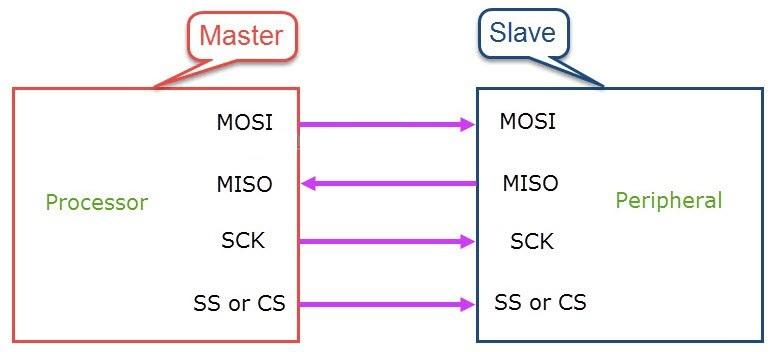
\includegraphics[scale=0.6]{images/SPI-One-Master-One-Slave.jpg}
\caption{Giao thức SPI giữa một master và một slave}
\label{fig:SPI_1M1S}
\end{figure}

\textbf{MOSI}, như tên cho thấy, là dữ liệu được tạo ra bởi master và nhận bởi slave.
Do đó, các chân MOSI trên cả master và slave được kết nối với nhau.

\textbf{MISO} là dữ liệu được tạo ra bởi slave và phải được truyền tới master.
Các chân MISO trên cả master và slave được kết nối với nhau.
Mặc dù tín hiệu trong MISO được tạo ra bởi slave, đường tín hiệu này được điều khiển bởi master.

Master tạo tín hiệu đồng hồ \textbf{SCK} và được cung cấp cho đầu vào đồng hồ của slave. Xung này có chức năng giữ nhịp cho giao tiếp SPI, vì SPI là chuẩn truyền đồng bộ nên cần 1 đường giữ nhịp, mỗi nhịp trên chân SCK báo 1 bit dữ liệu đến hoặc đi. Sự tồn tại của xung SCK giúp quá trình tuyền ít bị lỗi và vì thế tốc độ truyền của SPI có thể đạt rất cao.

Chip Select (CS) hoặc Slave Select (SS) được sử dụng để chọn một slave cụ thể bởi master.
Nếu master kéo đường SS của một slave nào đó xuống mức thấp thì việc giao tiếp sẽ xảy ra giữa master và slave đó.

Vì đồng hồ được tạo ra bởi master, luồng dữ liệu được điều khiển bởi master.
Với mỗi chu kỳ đồng hồ, một bit dữ liệu được truyền từ master đến slave và một bit dữ liệu được truyền từ slave đến master.

Quá trình này xảy ra đồng thời và sau 8 chu kỳ đồng hồ, một byte dữ liệu được truyền theo cả hai hướng và do đó, SPI là một giao tiếp song công toàn phần (full-duplex).

\subsection{UART}
\subsubsection{Giới thiệu}
Ngoài giao thức giao tiếp SPI, trong đề tài này còn có sử dụng giao tiếp UART để truyền tải dữ liệu đã xử lý với hai mục đích:
\begin{itemize}
    \item Mục đích chính dùng để debug chương trình trên máy tính khi thực hiện code trên vi xử lý thông qua cáp debug đi kèm cùng kit.
    \item Sau khi đã debug xong và chương trình ổn định, ta có thể dùng dữ liệu truyền tải từ UART để thực hiện xử lý dữ liệu một cách tự động sử dụng các ICs hoặc các modules khác.
\end{itemize}

Giao tiếp UART, tên đầy đủ là Universal Asynchronous Receiver/Transmitter, nó là một vi mạch sẵn có trong một vi điều khiển
nhưng không giống như một giao thức truyền thống (I\textsuperscript{2}C  và SPI).
Chức năng chính của UART là truyền dữ liệu nối tiếp.
Trong UART, giao tiếp giữa hai thiết bị có thể được thực hiện theo hai cách là giao tiếp dữ liệu nối tiếp và dữ liệu song song.

\begin{figure}[ht]
\centering
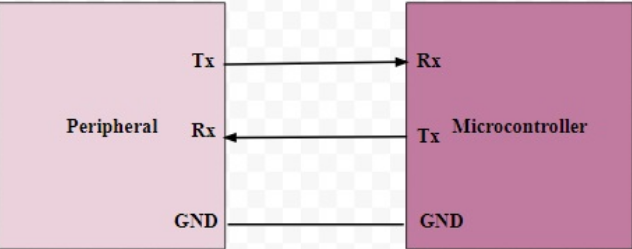
\includegraphics[scale=0.5]{images/UART_communication.png}
\caption{Giao tiếp UART}
\end{figure}

\subsubsection{Truyền thông nối tiếp và song song}
Trong giao tiếp dữ liệu nối tiếp, dữ liệu có thể được truyền qua một cáp hoặc một đường dây ở dạng bit-bit và nó chỉ cần hai cáp.
Truyền thông dữ liệu nối tiếp không đắt khi chúng ta so sánh với giao tiếp song song.
Nó đòi hỏi rất ít mạch cũng như dây.
Vì vậy, giao tiếp này rất hữu ích trong các mạch ghép so với giao tiếp song song.

Trong giao tiếp dữ liệu song song, dữ liệu có thể được truyền qua nhiều cáp cùng một lúc.
Truyền dữ liệu song song tốn kém nhưng rất nhanh, vì nó đòi hỏi phần cứng và cáp bổ sung.
Các ví dụ tốt nhất cho giao tiếp này là máy in cũ, PCI, RAM, v.v..

\begin{figure}[ht]
\centering
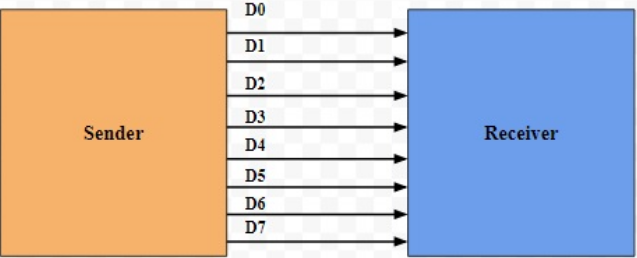
\includegraphics[scale=0.5]{images/UART_parallel.png}
\caption{Giao tiếp UART song song}
\end{figure}

\section{Giới thiệu phần mềm}
\subsection{Code Composer Studio}
\subsubsection{Giới thiệu}
Code Composer Studio (CSS) là một môi trường phát triển tích hợp (Integrated Đevelopment Environment - IDE)
hỗ trợ các kit và vi xử lý được sản xuất bởi Texas Instrument.
CSS bao gồm bộ công cụ sử dụng để phát triển và debug các phần mềm lập trình nhúng.
Một vài công cụ nổi trội có thể kể ra như: bộ phiên dịch C/C++ đã được tối ưu hóa cho từng vi điều khiển,
linker/loader được tích hợp sẵn, trình debugger, v.v..
CSS kết hợp sức mạnh của phần mềm Esclipse và bộ debugger, trình phiên dịch tối ưu hóa cho từng vi điều khiển
đã tạo nên một IDE hoàn thiện và mạnh mẽ cho việc lập trình phát triển nhúng cho vi điều khiển.

CSS hỗ trợ rất nhiều vi điều khiển khác nhau, từ dòng vi điều khiển cao cấp cho đến các dòng vi điều khiển tiết kiệm điện rẻ tiền, vi điều khiển thời gian thực C2000, SimpleLink Wireless, Sitara (Cortex-A \& ARM9), C3x/C4x/TMS320x DSPs, v.v..

Trong đề tài này, phiên bản CSS được sử dụng là 9.1.0.

\medskip
\subsubsection{Cài đặt}
Người dùng có thể đọc về cách cài đặt CSS bằng cách truy cập vào website chính thức của TI: \url{http://processors.wiki.ti.com/index.php/Download_CCS}

Ngoài ra, để lập trình phát triển phần mềm nhúng trên kit TIVA C một cách hiệu quả, người dùng được khuyến khích tải bộ thư viện \mintinline{bash}{TivaWare} từ website chính thức của nhà sản xuất: \url{http://www.ti.com/tool/sw-tm4c}

\subsection{serialport-rs}
Để đọc dữ liệu xuất ra từ UART của kit để debug ta có thể sử dụng thư viện \emph{serialport-rs}.
\emph{serialport-rs} là thư viện chuyên dụng cho việc xử lý thông tin từ Serial Port, được viết bằng ngôn ngữ lập trình Rust và hỗ trợ rất nhiều hệ điều hành khác nhau: Windows, MacOS/iOS, Linux, Android, FreeBSD, NetBSD, v.v..

Ngoài ra, người dùng có thể sử dụng trực tiếp công cụ \emph{Terimal} của CSS, tuy nhiên, ở đây tôi chọn \emph{serialport-rs} với mục tiêu sử dụng hệ thống RFID trên nhiều hệ thống, hệ điều hành khác nhau, không bị lệ thuộc vào công cụ CSS.

\medskip
\textbf{Cài đặt và sử dụng thư viện serialport-rs}:
\begin{enumerate}
\item Cài đặt ngôn ngữ Rust, xem thêm tại website chính thức: \url{https://www.rust-lang.org/tools/install}
\item Tải thư viện \emph{serialport-rs} từ link: \url{https://gitlab.com/susurrus/serialport-rs}
\item Build thư viện sử dụng lệnh build của công cụ cargo (đi kèm với bộ cài đặt của Rust):

\mintinline{bash}{$ cargo build --examples --release}
\item Sau khi đã build xong, ta kiểm tra thư viện đã được cài đặt đúng cách chưa bằng cách kết nối kit vào thiết bị (ở đây là máy tính) và chạy phần mềm \emph{hardware\_check} trên port giao tiếp với kit TIVA C: (ở đây là \mintinline{bash}{/dev/ttyACM0})

\mintinline{bash}{$ ./target/release/examples/hardware_check /dev/ttyACM0}
\item Nếu thư viện và thiết bị đều kết nối thành công và hoạt động bình thường thì thư viện sẽ trả về các kết quả kiểm tra thiết bị tương tự như hình \ref{fig:hardware_check_result}.
\end{enumerate}

Ngoài phần mềm IDE CSS và thư viện \emph{serialport-rs}, ta còn có thể sử dụng phần mềm \emph{lm4flash} từ bộ công cụ \emph{lm4tools} để có thể dễ dàng nạp chương trình đã thiết kế nhanh chóng trong môi trường CLI mà không cần dùng đến CSS.
Xem thêm tại link: \url{https://github.com/utzig/lm4tools}.

\newpage
\begin{figure}[ht!]
\centering
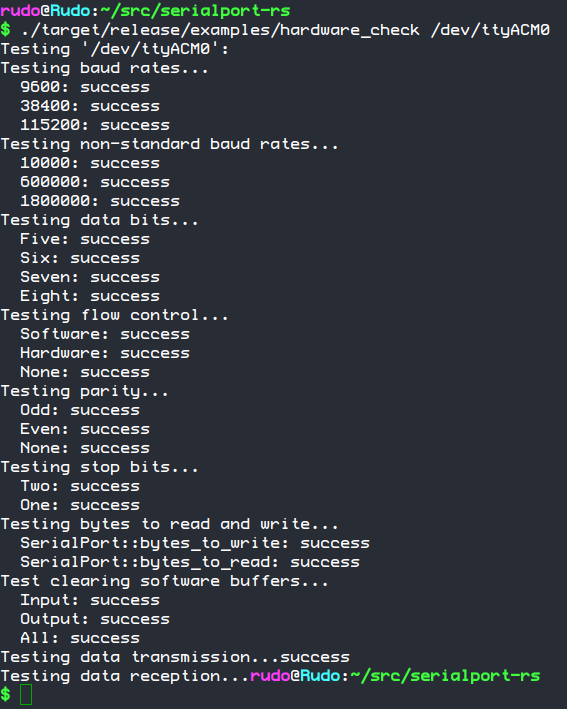
\includegraphics[scale=1]{images/hardware_check_result.png}
\caption{Kết quả kiểm tra kit TIVA C}
\label{fig:hardware_check_result}
\end{figure}

\newpage
\subsection{Sơ đồ khối và giải thuật của hệ thống}
\subsubsection{Sơ đồ khối hệ thống}
Hệ thống gồm 4 khối chính: khối đọc thẻ từ sử dụng module MFRC522,
khối vi xử lý sử dụng kit TIVA C, khối xuất kết quả gồm hai thành phần LCD 1602 và máy tính (hoặc các thiết bị khác).
Hệ thống có thể lấy nguồn từ dây cáp debug của kit kết nối vào máy tính hoặc nguồn 5V cấp từ bên ngoài.
Hình \ref{fig:system_diagram} biểu diễn sơ đồ của hệ thống RFID.
\begin{figure}[ht]
\centering
\begin{tikzpicture}[node distance=0.25cm and 1 cm]
\tikzset{block/.style = {draw, rectangle, align=center, minimum width=2cm, minimum height=1cm}, >= latex,}
% Main Nodes
\node (tiva) [block] {Kit TIVA C};
\coordinate[below=1cm of tiva] (empty1); % this is for drawing 90 degrees arrows
\node (lcd) [block] [right=3cm of tiva] {LCD 1602};
\node (MFRC522) [block] [left=3cm of tiva] {MFRC522};
\node (computer) [block] [below=1cm of lcd] {Máy tính};
\node (power) [block, minimum width=5cm] [below=2cm of empty1] {Nguồn cấp 5V};
\coordinate[right=4.5cm of power] (empty2); % This is for longer dashed box
% Naming Nodes
\node (tiva_n) [above=1cm of tiva] {Khối vi xử lý};
\node (lcd_n) [above=1cm of lcd] {Khối xuất kết quả};
\node (MFRC522_n) [above=1cm of MFRC522] {Khối đọc thẻ từ};
\node (power_n) [left=2cm of power, minimum height=1.5cm] {Khối nguồn};
% These corners are for drawing the big overall box
\coordinate[above left=0.5cm of MFRC522_n] (corner1);
\coordinate[below right=1.2cm and 0.3cm of empty2] (corner2);
% Draw dashed lines
\node[fit = (MFRC522_n) (MFRC522), dashed, draw, inner sep = 0.2cm] (box_rc522) {};
\node[fit = (tiva_n) (tiva), dashed, draw, inner sep = 0.2cm] (box_tiva) {};
\node[fit = (lcd_n) (computer), dashed, draw, inner sep = 0.2cm] (box_display) {};
\node[fit = (power_n) (empty2), dashed, draw, inner sep = 0.2cm] (box_power) {};
\node[fit = (corner1) (corner2), draw] (box_all) {};
% Connectors
\draw [->] (tiva) -- node[above, pos=0.45] {GPIOx6} (lcd);
\draw [->] (MFRC522) -- node[above] {SPI} (tiva);
\draw [->] (tiva) -- (empty1) |- node[above, pos=0.8] {UART} (computer);
\end{tikzpicture}
\caption{Sơ đồ khối hệ thống RFID}
\label{fig:system_diagram}
\end{figure}

\subsubsection{Giải thuật của hệ thống}\label{ref:algorithm}
\begin{enumerate}[label={Bước \theenumi.}, leftmargin=*, ref={\theenumi}]
    \item Đầu tiên, hệ thống khởi động (initialize) các cổng của vi điều khiển, điều chỉnh tốc độ vi xử lý,
        khởi động LCD, khởi động module MFRC522, v.v..
    \item Hệ thống chọn chip slave để đọc dữ liệu.
        Trong hệ thống này, chỉ có một slave được sử dụng nên nó là một khối đơn giản.
        Tuy nhiên, hệ thống có thể được phát triển lên để đọc dữ liệu từ nhiều slave khác nhau.
    \item LCD hiển thị dòng chữ ``Scan your card'' ra màn hình LCD, báo hiệu cho người dùng thực hiện quét thẻ.
        Đây là trạng thái mặc định của LCD, báo hiệu hệ thống đã sẵn sàng đọc một thẻ mới.\label{flow:lcd_default}
    \item Hệ thống kiểm tra xem có thẻ được quét hay không. Nếu không, hệ thống tiếp tục lặp cho đến khi đọc được thẻ mới.
        Nếu có thì chuyển sang bước \ref{flow:led_blink}.
    \item Vi điều khiển chớp LED xanh có sẵn trên board báo hiệu thẻ đã được đọc thành công.\label{flow:led_blink}
    \item Vi điều khiển xử lý dữ liệu đọc từ thẻ.
        Trong bước này, ta có thể điều chỉnh code để vi điều khiển kích hoạt relay để mở cửa, chạy động cơ, v.v..
    \item Vi điều khiển xuất kết quả ra LCD và UART và quay lại bước \ref{flow:lcd_default}.
\end{enumerate}

\bigskip
Hình \ref{fig:flow_chart} mô tả lưu đồ giải thuật của hệ thống RFID.
\begin{figure}[ht]
\centering
\begin{tikzpicture}
\tikzset{startstop/.style = {draw, rectangle, rounded corners, align=center, minimum width=3cm, minimum height=1cm}, >= latex,}
\tikzset{process/.style = {draw, rectangle, align=center, minimum width=3cm, minimum height=1cm}, >= latex,}
\tikzset{decision/.style = {draw, diamond, align=center, minimum width=3cm, minimum height=1cm}, >= latex,}
% Main nodes
\node (start) [startstop] {Bắt đầu};
\node (init) [process] [below=1cm of start] {Initialize hệ thống \\ Chọn chip slave};
\node (lcd_default) [process] [below=1cm of init] {Hiển thị dòng chữ \\ "Scan your card" ra LCD};
\node (card_check) [decision] [below=1cm of lcd_default] {Kiểm tra \\ có thẻ \\ được quét \\ không?};
\node (led_blink) [process] [below=1cm of card_check] {Chớp LED trên board \\ báo hiệu đã đọc thẻ};
\node (data_process) [process] [below=1cm of led_blink] {Xử lý dữ liệu \\ đọc từ thẻ};
\node (data_output) [process] [below=1cm of data_process] {Xuất kết quả ra \\ LCD và UART};
% Various coordinates
\coordinate[left=2cm of data_output] (left_out);
\coordinate[above=0.5cm of card_check] (loop);
\coordinate[right=1cm of card_check] (right_card);
\coordinate[right=1cm of loop] (right_loop);
% Connectors
\draw [->] (start) -- (init);
\draw [->] (init) -- (lcd_default);
\draw [->] (lcd_default) -- (card_check);
\draw [->] (card_check) -- node [left] {Y} (led_blink);
\draw [->] (card_check) -- node [above] {N} (right_card) |- (right_loop) |- (loop);
\draw [->] (led_blink) -- (data_process);
\draw [->] (data_process) -- (data_output);
\draw [->] (data_output) -- (left_out) |- (lcd_default);
\end{tikzpicture}
\caption{Lưu đồ giải thuật của hệ thống RFID}
\label{fig:flow_chart}
\end{figure}
